\documentclass[conference]{IEEEtran}
\IEEEoverridecommandlockouts
% The preceding line is only needed to identify funding in the first footnote. If that is unneeded, please comment it out.
\usepackage{cite}
\usepackage{amsmath,amssymb,amsfonts}
\usepackage{algorithmic}
\usepackage{graphicx}
\usepackage{textcomp}
\usepackage{xcolor}
\usepackage{makecell}

\usepackage{multirow}
\usepackage{rotating}

\usepackage{mdframed}
\usepackage{hyperref}
\usepackage{tikz}
\usepackage{makecell}
\usepackage{tcolorbox}
\usepackage{amsthm}
%\usepackage[english]{babel}
\usepackage{pifont} % checkmarks
%\theoremstyle{definition}
%\newtheorem{definition}{Definition}[section]
\usepackage{svg}

\usepackage{listings}
\lstset
{ 
    basicstyle=\footnotesize,
    numbers=left,
    stepnumber=1,
    xleftmargin=5.0ex,
}


%SCJ
\usepackage{subcaption}
\usepackage{array, multirow}
\usepackage{enumitem}


\def\BibTeX{{\rm B\kern-.05em{\sc i\kern-.025em b}\kern-.08em
    T\kern-.1667em\lower.7ex\hbox{E}\kern-.125emX}}
\begin{document}

      
\title{Research on architectural challenges for Industry~4.0 systems through the development of a~production system\\
}

\author{
    \IEEEauthorblockN{
        Henrik Schwarz\IEEEauthorrefmark{1},
        Hampus Fink Gärdström\IEEEauthorrefmark{1},
        Fahim Shahriar\IEEEauthorrefmark{1},
        Tom Bourjala\IEEEauthorrefmark{1},
        Tomas Soucek\IEEEauthorrefmark{1},
        Henrik Prüß\IEEEauthorrefmark{1}
    }
    \IEEEauthorblockA{
        University of Southern Denmark, SDU Software Engineering, Odense, Denmark \\
        Email: \IEEEauthorrefmark{1} \textnormal{\{hschw17,hgard20,fasha23,tobou23,tosou23,hepru23\}}@student.sdu.dk
    }
}



\maketitle
\IEEEpubidadjcol
\begin{abstract}
%%%%%%%%%%%%%%%%%% Max 970 signs without space %%%%%%%%%%%%%%%%%%

% Intro
In this paper an architecture for a fictional use case of an automated industry 4.0 bike factory was proposed to investigate how architecture design can support a production systems and what trade-offs arise in Industry 4.0 environments.

% Gab
Development of software systems involving Industry 4.0 imposes many architectural constrains that must be considered. Different technological choices impact how the system can be designed in a way that builds around these architectural constraints. However, different technological choices and the design of a system has trade-offs. What these trade-offs are, or how they are dealt with, is not clear from current research.  

% Aim 
The aim of the study is to investigate these trade-offs and analyze how different architectures can support a set of system requirements.

% Method
The bike factory case was analysed which resulted in four main quality attributes being scalability, interopability, maintainability and deployability that were used to design to design an overall system and a smaller architectural prototype which were later tested and verified using time as measurement with two experiments.
 
% Results
The experiments verified the deployment strategy and gave a~interesting insight the scalability of the system. The scalability expiriment raised some new questions that would be answered in future work. The process of using quality attributes and quality attribute scenarios to create the system also needs further investigation.

\end{abstract}

\begin{IEEEkeywords}
I4.0, Software Architecture, Quality Attribute, Software Engineering
\end{IEEEkeywords}

\section{Introduction and Motivation}
%Introduction and motivate the problem
The rise of Industry 4.0 has created a need for the development of more complex and interoperable systems. Building these systems is challenging and poses architectural challenges. Many of these challenges stem from the many different interconnecting components. The Industry 4.0 faces particular challenges in integrating a variety of technologies, services, and components. This integration not only complicates the system but also restricts its architectural flexibility. Additionally, systems often have additional non-functional requirements which further complicate development. Notably, there is often a need for scalability and high availability in such systems, which requires developers to consider and design their systems around these requirements. 

All these factors raise the need for methods that help to develop systems in a way that they fulfill defined quality attributes (QA).

The structure of the paper is as follows. 
Section \ref{sec:problem} outlines the research question and the research approach. 
%to analyze the research question and evaluate our results.
Section \ref{sec:related_work} describes similar work in the field and how our contribution fits the field.
Section \ref{sec:use_case} presents a production system use case.
The use case serves as input to specify QA requirements in Section \ref{sec:qas}.
Section \ref{sec:middleware_architecture} introduces the proposed production system software architecture design.
Section \ref{sec:evaluation} evaluates the proposed system and analyzes the results against the stated QA requirements.   

\section{Problem and Approach}

\label{sec:problem}
\emph{Problem.}
In this paper architectural challenges are explored through the development of architectural prototypes for a~flexible production system for an assembly line. Production systems typically contain many different components. In this assembly line production system, the interaction of multiple components is essential for supporting a common task.

The context of this production system is a fictional bike manufacturing company. The fictional company produces bikes that are highly customizable and rapidly produced on-demand. The production line should have the least downtime in order to constantly produce bikes. Moreover, it should be able to scale in order to handle increased production demands. The high customizability demands a greater need for interoperability.    
  
\emph{Research questions:}
\begin{enumerate}
    \item  How can different architectures support the production systems requirements?
    \item  Which architectural trade-off must be taken due to the technology choices?
\end{enumerate}


\emph{Approach.}
The following steps are taken to answer this paper's research questions: 
\begin{enumerate}
    \item Research-related work
    \item Define use cases and quality attribute scenarios
    \item Design and implement prototypes of the system architecture
    \item Perform scenario experiments
    \item Analyze and evaluate results
\end{enumerate}

\section{Related work}
\label{sec:related_work}

There is a considerable amount of literature on quality attributes in the research field of software architecture. For instance, multiple sources provide a general overview of quality attributes, and how they are used to define and evaluate a software system’s architecture \cite{barbacci_quality_1995}\cite{bass2012software}. More specifically, a paper \cite{offutt_quality_2002} shows how quality attributes are used to evaluate web software applications, while another \cite{obrien_quality_2007} focuses on the quality attributes of service-oriented architectures.

In the context of Industry 4.0 (I4.0), there are a few examples of using quality attributes to evaluate software architectures. A study\cite{antonino_quality_2022} was found that provides a quality model, based on the ISO/IEC 25010 standard \cite{noauthor_isoiec_2011}, to identify quality attributes in I4.0 software architectures. The proposed quality model is applied to two operational Industry 4.0 software architectures to verify its suitability.

The article \cite{thramboulidis_cyber-physical_2018} investigated the use of the microservice architecture in the I4.0 domain. Therefore, the authors conducted an experiment on a production system, transforming physical production machines into cyber-physical microservices that communicate over a network. Due to the microservice architecture, production machines can be added and removed, as required by the production schedule. The authors find that the use of microservice architecture increases the flexibility of the production system, thereby addressing the quality attribute of deployability. \cite{thramboulidis_cpus-iot_2019} expanded on the idea by providing a framework for integrating microservices into I4.0 production systems.

Another paper \cite{jepsen_industry_2021} analyzed the requirements of middleware used for connecting different production machines in I4.0 software architectures. The analysis is conducted based on the Level of Conceptual Interoperability Model (LCIM), and concludes that middleware of I4.0 applications needs to consider the different levels of interoperability to ensure successful coordination and communication between the different production machines, thus addressing the interoperability quality attribute.

In \cite{jepsen_reconfigurable_2023}, a software architecture addressing the quality attribute of reconfigurability in the domain of Industry 4.0 was presented. The proposed architecture is based on an event-driven architecture and utilizes an orchestrator, a central message bus, and several services to enable coordination and communication of the production machines. Furthermore, the paper describes a reconfigurable quality attribute scenario to verify the usefulness of the proposed architecture.

A systematic mapping of I4.0 architecture \cite{hofer_architecture_2018} showed that some fields of study like integration and information management gain the researchers' attention, while other fields like reconfiguration or verification and validation are under-investigated. As concluded in \cite{pivoto_cyber-physical_2021}, more research is needed to discover the potentials of recent trends like cloud computing or big data processing for I4.0 architectures, e.g. for handling the vast amount of data being produced by sensors and other IoT devices that are involved in the Industry 4.0. Such research would address the quality attributes of performance, scalability, and availability.

The contribution of this particular paper is to design architectural prototypes of I4.0 systems that address different quality attributes. While this has been done by others before \cite{jepsen_industry_2021} \cite{jepsen_reconfigurable_2023}, the study stands out by addressing multiple quality attributes at the same time. This can be especially beneficial in real-world applications because I4.0 systems usually have to fulfill multiple quality attributes at the same time, introducing the necessity for trade-offs between different attributes. Like \cite{bachmann_designing_2005} does in a generic context, the study aims towards quality attributes shaping software architecture in the specific I4.0 context.

\section{Use Case and Quality Attribute Scenario}
\label{sec:use_case_and_qas}
This Section introduces specific use cases and their associated quality attribute scenarios used for the experiment. The quality attribute scenarios are developed based on the use cases.

\subsection{Use case}
\label{sec:use_case}

Two use cases were selected for their relevance and their potential for highlighting architectural requirements.

\begin{figure}
    \centering
    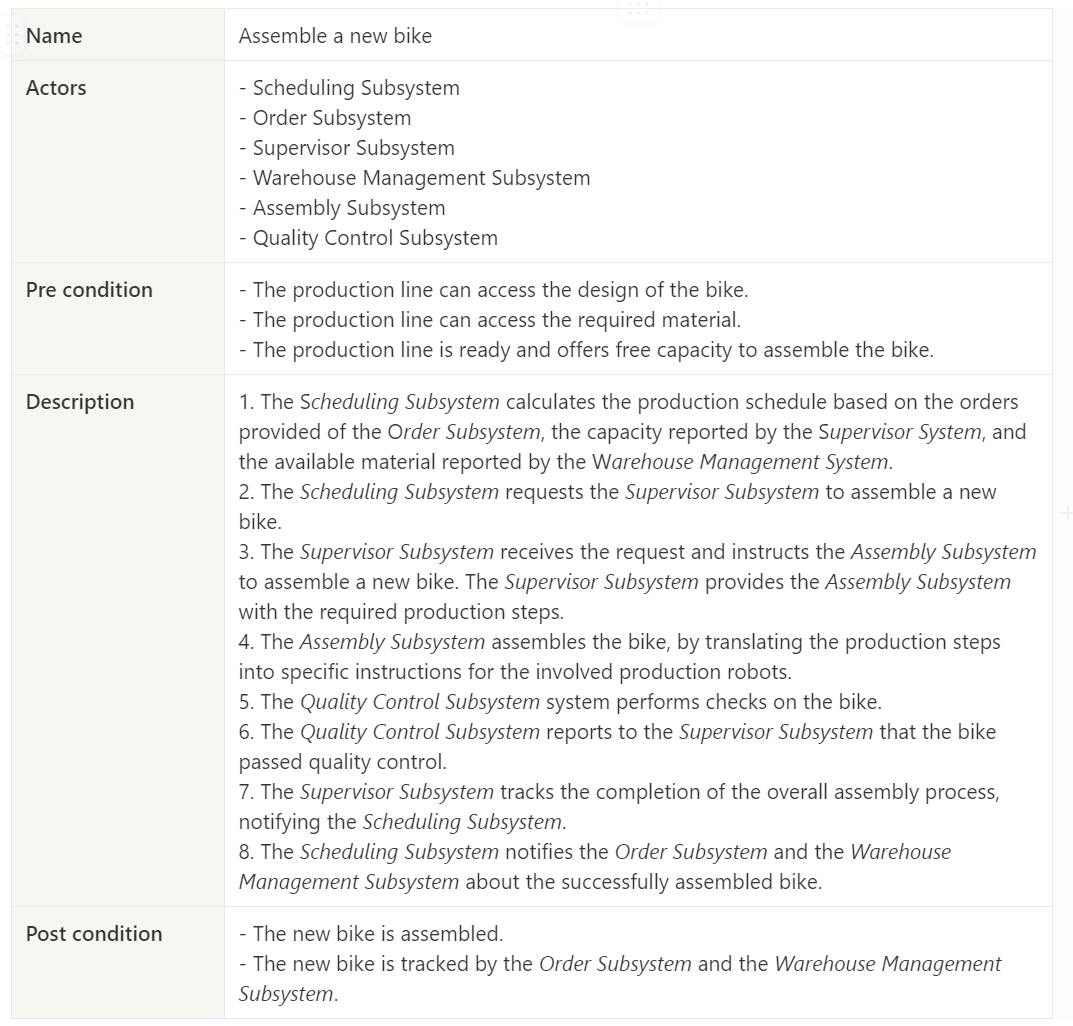
\includegraphics[width=1\linewidth]{img/UC Assemble a new bike.png}
    \caption{Assembly of a new bike}
    \label{fig:UC: Assemble of a new bike}
\end{figure}

The first of those use cases was the assembly of a new bike \ref{fig:UC: Assemble of a new bike}. This characterizes the core and main purpose of the endeavour, which is to produce bikes on-demand. This is interesting because assembling a bike and tracking its status is a complex process which would involve multiple (software) systems if implemented as an I4.0 system, including:
\begin{itemize}
    \item The \textit{Order Subsystem}, which keeps track of the orders and serves as an interface between the user interface and the multiple systems.  
    \item The \textit{Scheduling Subsystem}, which schedules and tracks the production of the bike based on the \textit{Order Subsystem} requests. 
    \item The \textit{Supervisor System}, which oversees the production steps, including the \textit{Assembly Subsystem} and the \textit{Quality Control Subsystem}. 
\end{itemize}

This use case illustrates and lists the interactions and behaviour of the listed systems, effectively highlighting the main communication path required by the architecture. 
While the use case describes the production of one unit, it is reasonable to expect multiple units to be produced at the same time. The simultaneous execution of multiple instances in this use case underscores the importance of scalability for both the \textit{Supervisor Subsystem} and the \textit{Assembly Subsystem}, given their significant workload and activity in this context.

\begin{figure}
    \centering
    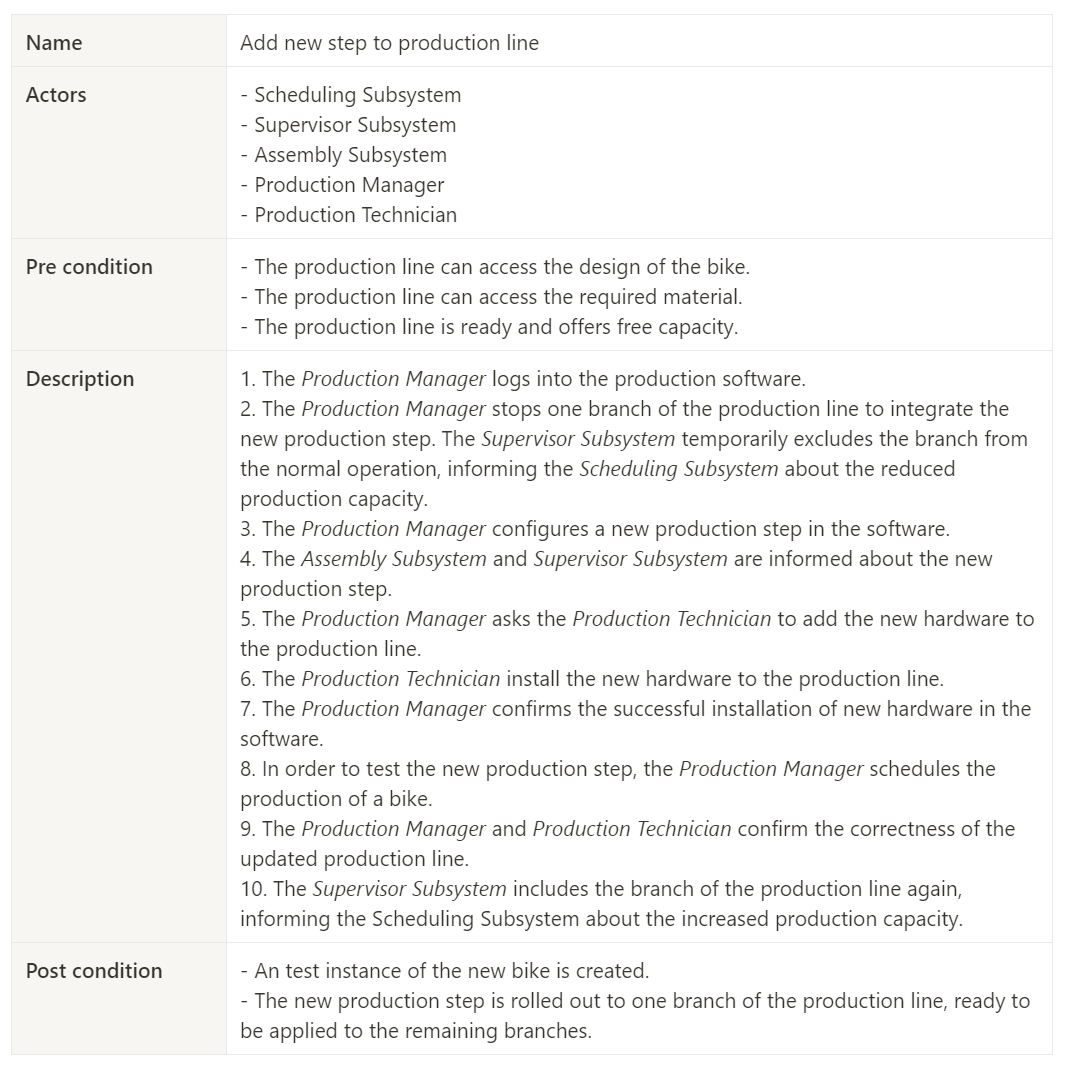
\includegraphics[width=1\linewidth]{img/UC Add new step to production line.png}
    \caption{New step to the production line}
    \label{fig:UC: New step to production line}
\end{figure}

The second selected use case is the addition of a step in the production line \ref{fig:UC: New step to production line}. It showcases how the assembly ecosystem needs to interact and respond to the administrator altering the configuration, in this case adding a production step. By describing how the editing and updating pipeline should take place, this use case illustrates another quality attribute that the system needs to exhibit: \textbf{\textit{Deployability}}. Automating the pipeline of software deployment is key for the system, as it would include multiple complex manipulations in order to minimize disruption of the production, which should work 24/7. This automation also allows for a short time from validation to production, which is valuable as changes on the production line, such as adding a new step, need to be quickly integrated to the production line.


\subsection{Quality attribute scenarios}
\label{sec:qas}

As the use cases illustrate the need for specific quality attributes, two measurable quality attribute scenarios were developed [\ref{fig:QAS Scalability}, \ref{fig:QAS Deployability}]. They were designed as a reference to ensure that the architecture can meet the requirements.

\begin{figure}
    \centering
    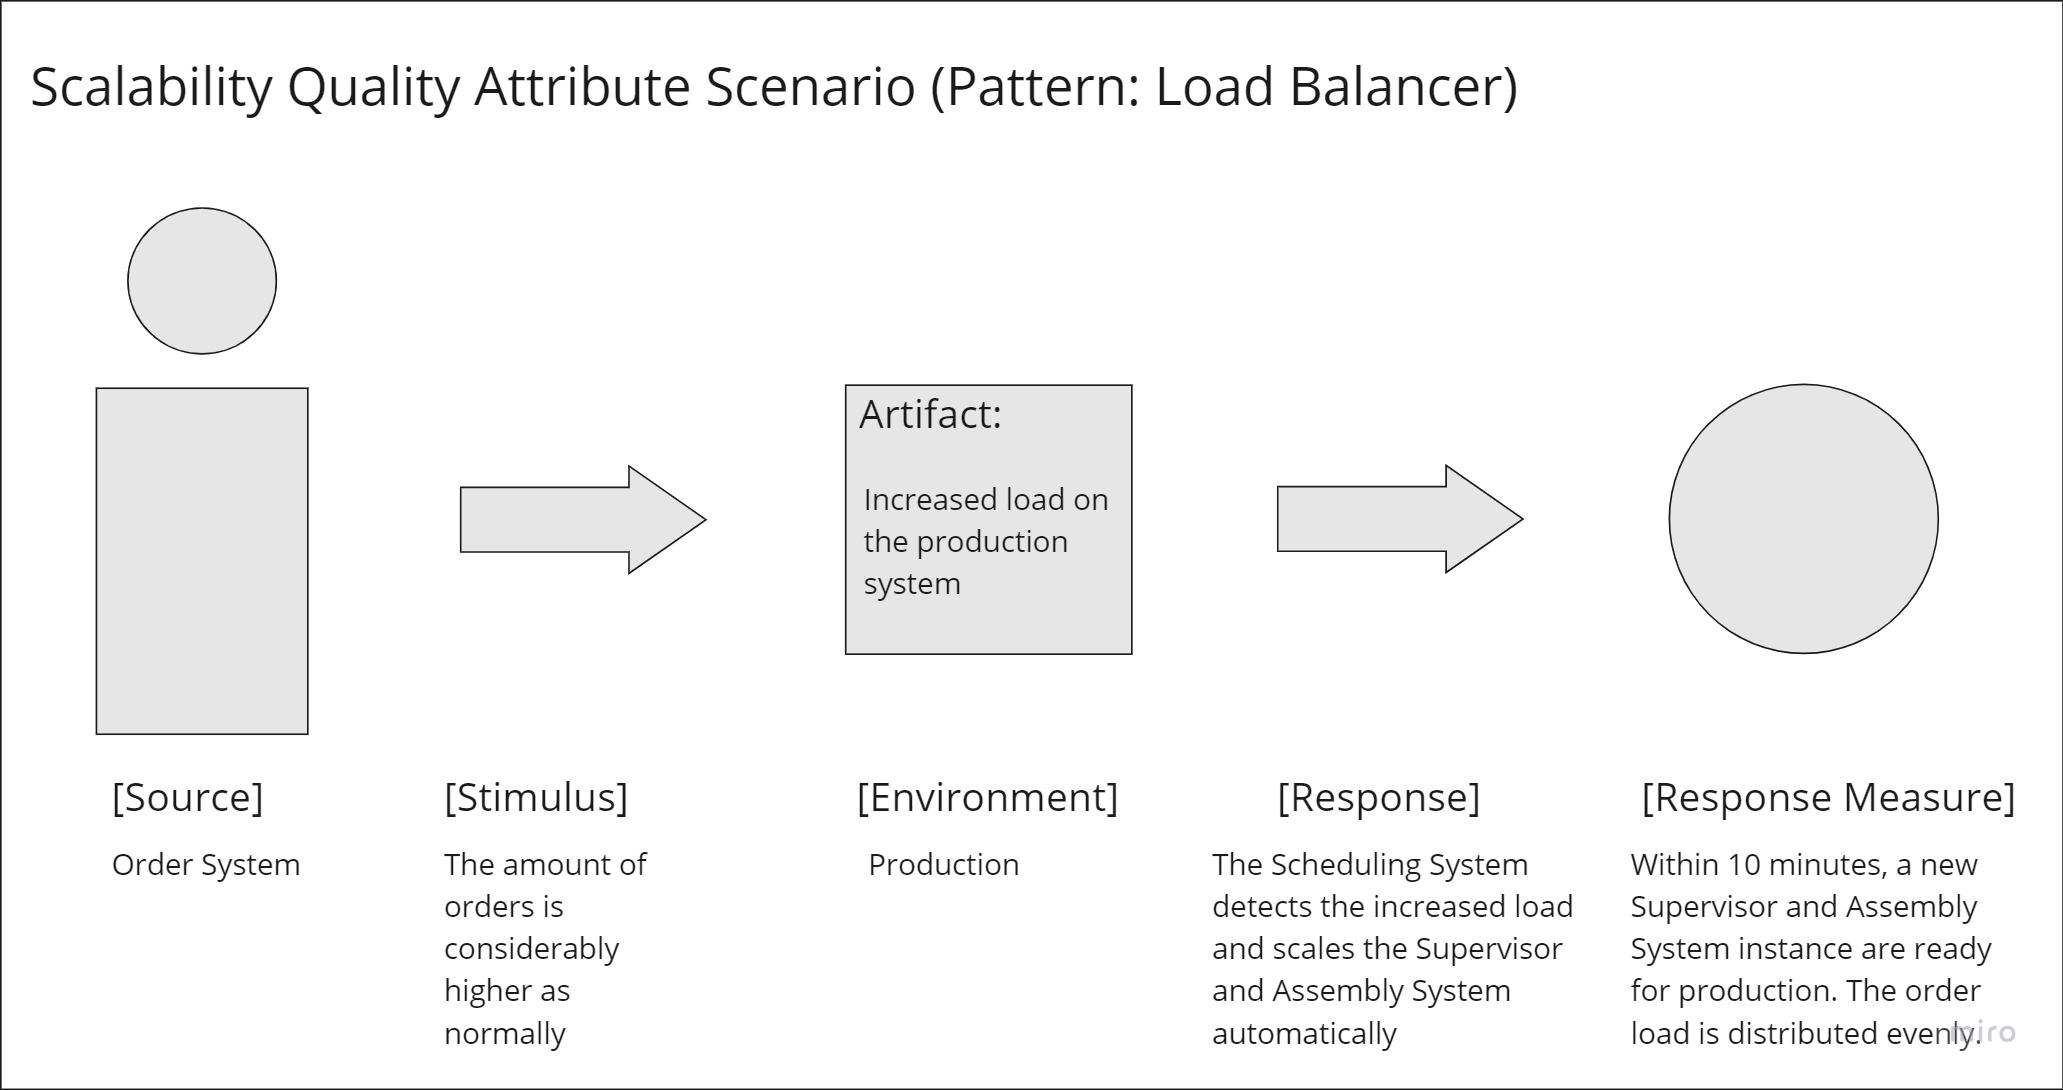
\includegraphics[width=0.9\linewidth]{img/QAS Scalability.png}
    \caption{Scalability Quality Attribute Scenario}
    \label{fig:QAS Scalability}
\end{figure}

For the first use case, describing the production of a new bike, fig. \ref{fig:UC: Assemble of a new bike},
a system was designed to use a \textbf{\textit{Load Balancer Pattern}} in order to achieve the \textbf{\textit{Scalability}} quality attribute. Scalability is required to meet the changing demand and adapt the resources employed to the load on the systems. If only a few bikes are to be produced, a minimal amount of systems (and production lines) should be put in motion to reduce power consumption, maintenance cost, and complexity. However if a large batch needs to be produced in a short period, then a proportional amount of systems should be put into motion to meet the demand. The \textbf{\textit{Load Balancer}} automatically balances the load between multiple \textit{Supervisor} and \textit{Assembly} subsystems instances according to the number of orders waiting to be processed. Those requirements for the \textit{\textbf{Load Balancer}} is illustrated in the scalability quality attribute scenario (figure \ref{fig:QAS Scalability}).

\begin{figure}
    \centering
    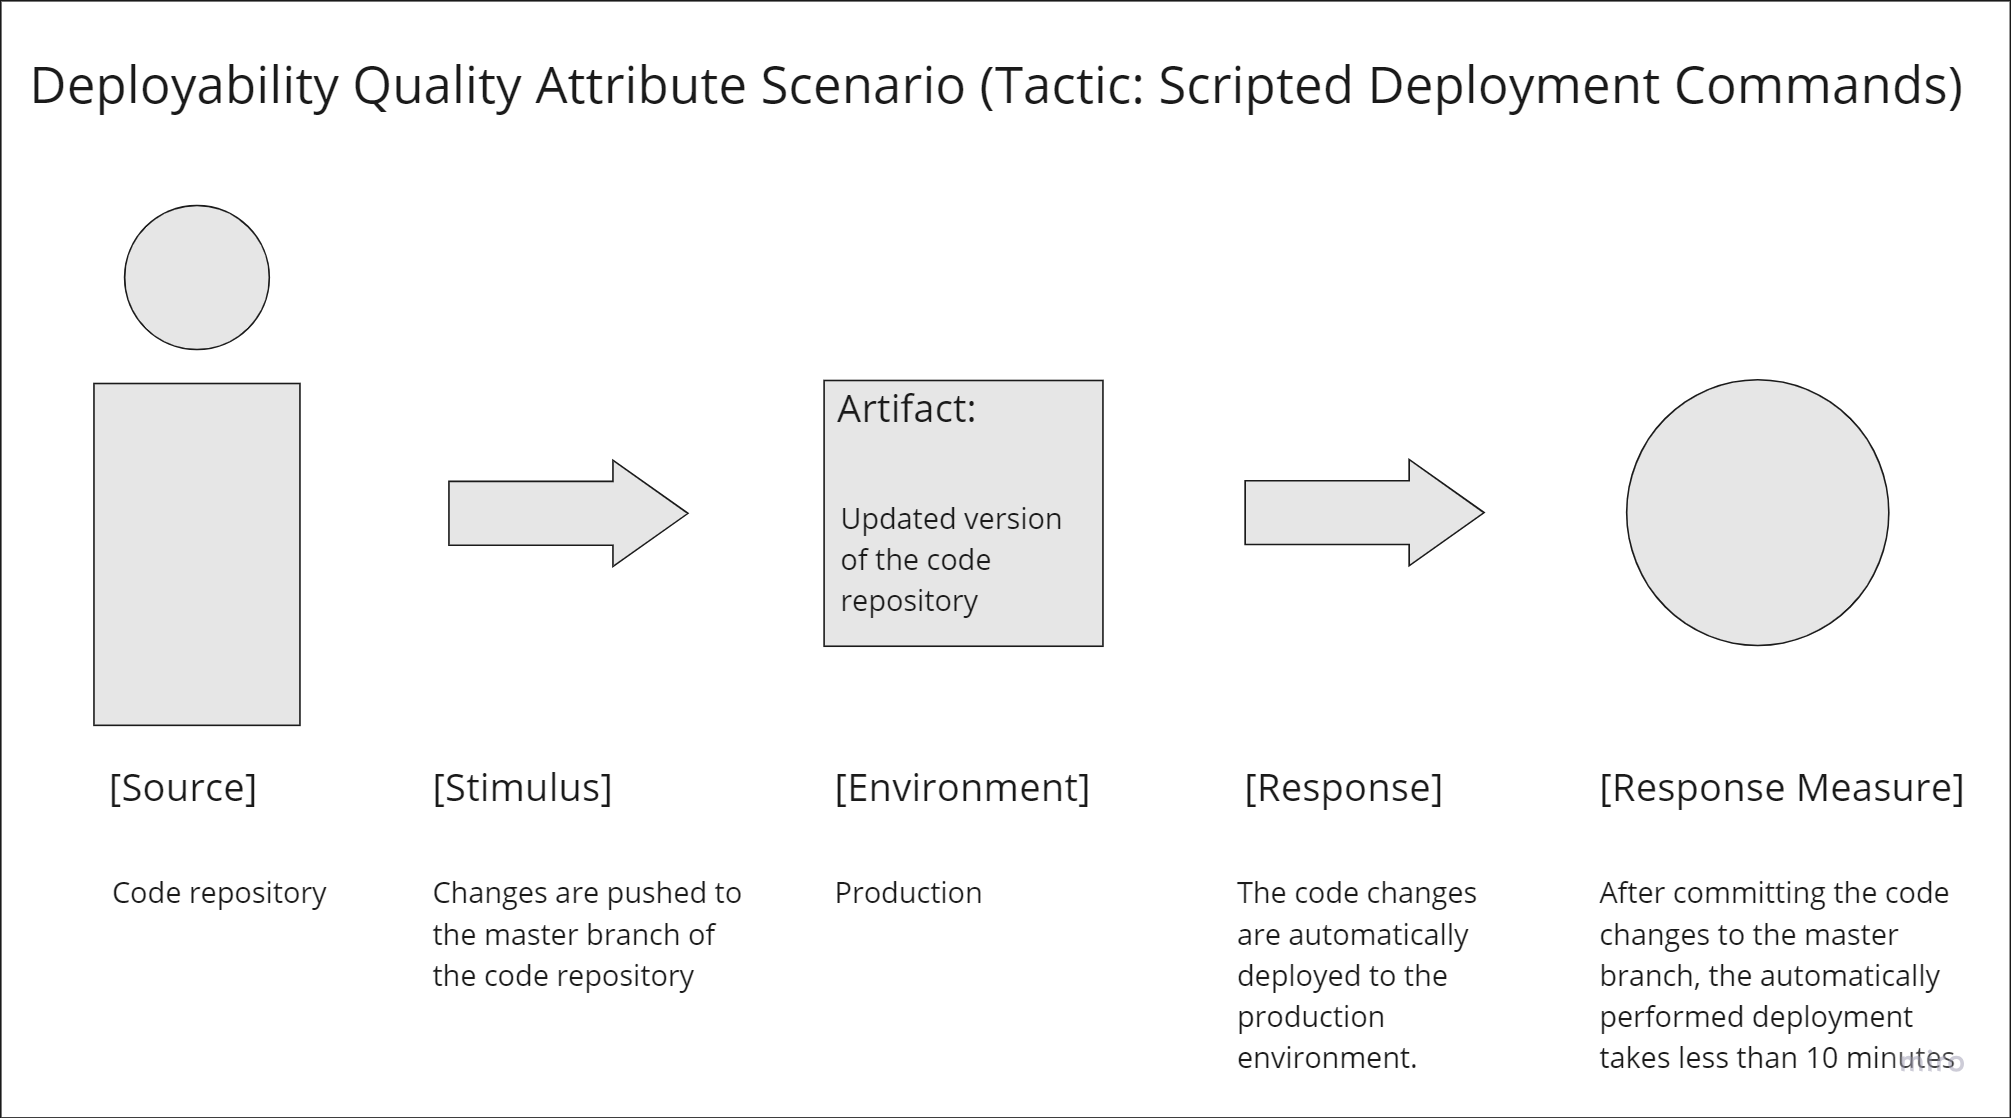
\includegraphics[width=0.9\linewidth]{img/QAS Deployability.png}
    \caption{Deployability Quality Attribute Scenario}
    \label{fig:QAS Deployability}
\end{figure}

For the second use case, describing the addition of a new step to the production pipeline \ref{fig:UC: New step to production line}, a \textbf{\textit{Scripted Deployment Command}} strategy was employed to meet the architectural requirement and achieve the \textbf{\textit{Deployability}} quality attribute. 
The deployability quality attribute scenario \ref{fig:QAS Deployability} is designed to describe how the system should react to changes to the code repository. 

\section{The solution}
\label{sec:middleware_architecture}

This section will describe a proposed architecture that aims to achieve the stated requirements, addressing the first research question. The proposed design is then partially implemented as architectural prototypes.

\subsection{Systems}
The overall solution consists of 3 main systems that handle all tasks from receiving orders to production and supply chain management. Namely, the solution is made up of enterprise resource planning (ERP), supply chain management, and production management systems. The aim of this chapter is to describe a production management system, that was selected for deeper research and implementation. It has been opted for this system because its connection to Industry 4.0 is believed to be the closest, as this system handles the communication of production machines, scheduling, and other production-related tasks. It consists of 4 different subsystems, that are mentioned in table \ref{tab:subsystem}.

\begin{table}[htbp]
\caption{The Subsystems of the Production Management System}
\begin{center}
\begin{tabular}{|l|l|}
\hline
\textbf{Subsystem name}  & \textbf{Responsibilities} \\ \hline
Scheduling              & \makecell[l]{Based on orders from the ERP system,\\ decide when to schedule product manufacturing.\\Send instructions to the assembly subsystem.}   \\ \hline
Quality Control       & \makecell[l]{Checks for quality of parts and the whole bike\\ using cameras and other sensors. Report to the\\ supervisor subsystem.}          \\ \hline
Supervisor              & \makecell[l]{Monitors and supervises the system. Keeps track of\\ the status of the production line. Gives instructions \\to assembly subsystem to circumvent hardware\\ malfunction and safety hazards.}        \\ \hline
Assembly            & \makecell[l]{Translates the orders from the scheduling to the \\robots, and reports back to the supervisor system\\ with estimated time of arrival updates.}      
            \\ \hline
\end{tabular}
\end{center}
\label{tab:subsystem}
\end{table}

Figure \ref{fig:communicationDiagram} shows a communication diagram between the supervisor, assembly, and quality control subsystems. The quality control subsystem was not implemented in the final solution and was only left in the graph, to provide a better understanding of communication steps and to demonstrate usage of an AMQP message broker. This broker was picked because of its non-blocking asynchronous requests and high availability. In the case of an error, AMQP allows for rigorous error handling (as described in its specification \cite{amqpDoc}), allowing the proposed architecture to react properly and recover.

In the figure \ref{fig:communicationDiagram}, it is also possible to see different programming languages for different parts of subsystems. To begin with a Supervisor subsystem, it has been decided to split front-end and back-end implementation. This separation allows for a visualization of inner processes and is an endpoint for user interaction with the whole production system. For front-end, a lightweight JavaScript framework called Svelte has been used. Svelte is a compiled and compact JavaScript solution that excels in performance. The back-end is handled by Spring Boot, a popular Java framework aiming to simplify the creation of stand-alone applications. Spring Boot was also selected for the assembly subsystem. 

Instructions for production cells are stored as a part of the assembly subsystem in S3 bucket storage. This blob storage is believed to be a great suit for instruction files because their structure can vary a lot and finding a common schema could be inefficient. Data exchanged between supervisor and assembly subsystems are stored in MongoDB, whose strength is a flexible schema possibility and fast read and write operations. To be able to save big amounts of logs in a very efficient manner, another database was introduced to the system. It has been opted for InfluxDB since it was built for time-series data, and that is a field into which systems logs fit greatly.

\begin{figure}
 \centering
 \includesvg[width=0.5\textwidth]{img/system-communication}
 \caption{Communication diagram between Supervisor, Quality Control, and Assembly subsystems}
 \label{fig:communicationDiagram}
\end{figure}

The selected systems were containerized using Docker. This adoption enhances scalability through easy management of horizontal scaling using different amounts of replicas. Docker also promotes a modular and encapsulated approach to software deployment, which makes it easier to update and maintain individual components without affecting the entire system. It also facilitates versioning of container images positively affecting system´s traceability. Potentially the part, for which Docker is used commonly, is in terms of interoperability and deployability quality attributes. Docker provides a standardized packaging format, making it easier to deploy applications consistently across different environments. Interoperability is enhanced by encapsulation of the application and its dependencies using containers.

\subsection{Addressed quality attributes}
The quality attributes that are promoted by the system architecture are scalability, interoperability, maintainability, and deployability. The selected quality attributes derive from earlier discussions driven by the created system context (e.g. assumptions, use cases).

\subsubsection{Scalability \& performance}
Scalability and performance in the described system are achieved primarily through two means. First, by leveraging brokers between services to facilitate scalable communication. Second, by ensuring that all of the communicating services can run with multiple instances at the same time, leading to the possibility of horizontal scaling. Regarding these two quality attributes, several design patterns have been used.

First to be mentioned is the extensive use of the \textbf{Microservice} pattern. The systems architecture uses the design pattern to create independent (sub-)systems with a single responsibility. For example, the production line is comprised of four Microservices (see table \ref{tab:subsystem}) instead of one monolith. This is beneficial if the load of only a single subsystem increases while staying the same for others. Instead of having to scale a monolith, one can scale selected subsystems saving resources and addressing only the part under load. For this pattern, the implementation challenges include slicing the system into sensible Microservices that are the proper size, and the choreography of the Microservices.

Another helpful pattern is the \textbf{Publisher/Subscriber}. This approach provides the system with non-blocking event-driven architecture improving system responsiveness. The supervisor subsystem listens to messages being produced by the assembly subsystem and uses them to calculate the supervision over the production line, allowing it to load balance incoming production jobs and distribute them to the production machines. Since the implementation of the pattern heavily relies on the AMQP message broker, potential disruption can come in the form of a broker being a bottleneck. The use of brokers and publisher/subscriber pattern also supports the limit dependencies tactic, in terms of integrability.

\subsubsection{Maintainability}
Regarding maintainability, the \textbf{Microservice} design pattern promotes the single responsibility principle. The clear separation of concerns between the components helps the maintainability purposes, as each Microservice only serves one purpose. The locating of the code of a certain feature becomes easier. Microservices also help with system decoupling, hence maintaining and developing the code becomes more straightforward. However, the associated challenge of using the design pattern remains in finding the right balance in the size of different services. Furthermore, Microservices can impact the traceability and testability of the overall system negatively. Features might span across multiple Microservices with each having its own logs. Thus, in order to trace a single feature, developers have to inspect multiple log files at the same time and combine their meanings. The same applies to the testing because again features are distributed among multiple Microservices. End-to-end testing of such architecture requires the orchestration of the microservices that are related to the tested feature, which increases the overall complexity of the test setup.

\subsubsection{Interoperability}
Even though both supervisor back-end and assembly server are using Java, a JSON data format was selected for communication. This means that communication does not rely on the use of a specific programming language, and any part of the system can be changed at any time. This approach makes it easier to swap components, allowing for more flexibility in system deployment and updates. Regarding Interoperability, the design solution counts with the need for a middleware layer helping to translate different outer data formats into the inner one. For this purpose, the \textbf{Adapter} design pattern was proposed. This pattern helps to connect systems using different interfaces or file formats by acting as a middleware, that converts from one format to another. It is particularly the assembly subsystem that benefits from the Adapter pattern, because it involves production machines from different vendors, each coming with their own set of interfaces and file formats. However, the Adapter pattern still requires the implementation of the adapter to be performed by a developer. If the production machines are replaced regularly, the Adapter pattern might reduce, but not eliminate the integration time. Therefore, the challenge is to engineer a~reusable implementation that only requires slight adjustments for each production machine.

\subsubsection{Deployability}
Another quality attribute addressed by the proposed architecture is deployability. As for other quality attributes, the \textbf{Microservice} architecture pattern helps to achieve deployability. Because the production system is split into four subsystem with each subsystem being a Microservice, different parts of the system can be deployed independently. If, for instance, the supervisor subsystem must be updated, a new version of it can be deployed while the old deployments of the other subsystems can be retained. Re-deploying only the system parts that changed reduces the deployment time and saves resources. Moreover, it reduces the risks involved with deployments because only parts of the system are temporarily unavailable within the deployment process.

Architectural tactics as proposed by Bass \cite{bass2012software} are employed to improve the system's deployability. Code changes that are merged with the main branch are automatically deployed to the production environment to achieve continuous delivery, i.e. tactic 'Scripted Deployment Commands'. By automating the deployment process the risk of manual errors is reduced. If faulty code changes are deployed to the production environment, they are automatically rolled back to the last working version of the code base. In order to achieve that behavior, the architecture relies on heartbeat messages that indicate a~working environment. If no heartbeat messages are received by a service, the central coordinator initiates the rollback of the specific service, i.e. tactic 'Rollback'.


\section{Evaluation}
\label{sec:evaluation}
In order to evaluate the proposed software architecture, several experiments were conducted. The scalability of the architecture was tested by horizontally scaling one of the subsystems and measurements of the resulting delivery time of messages between multiple subsystems. The deployability of the architecture was tested by creating a pipeline that automatically deploys new versions of the system, reducing the need for manual intervention. Pilot tests were not conducted, as the scope and labor involved in the the experiments were small to the extent that a preliminary test was not needed.
Both experiments were described and analyzed in the section, thereby following the same subsection structure: Section \textit{Experiment design} introduces the design of the experiment to evaluate the system. Section \textit{Measurements} identifies the measurements in the system for the according experiment. Section \textit{Analysis} presents the analysis of the results from the experiment.

\subsection{Experiment A - Scalability}
 
\subsubsection{Experiment design}
\label{sec:design}

The experiment addressing the scalability quality attribute was driven by the previously mentioned quality attribute scenario \ref{fig:QAS Scalability}. It was simulated that the assembly subsystem, controlling the production machines, sends sensor data to the supervisor subsystem every second. The supervisor uses the received sensor data to monitor the overall production progress. In case of errors, the supervisor can re-calculate the production plan and send new instructions to the assembly subsystem.

The described scenario involved the assembly subsystem, the supervisor subsystem and a message broker between those two systems. Also, a time series database was utilized to persist the sent messages. The conducted experiments investigated how the delivery time of messages between the systems changes, when the supervisor subsystem is horizontally scaled, i.e. when more container instances of the supervisor subsystem are added. While the mentioned quality attribute scenarios describe automated scaling, the scaling in the experiment happens manually. This should still allow for valid results as it is investigated whether or not the supervisor system is fit to be horizontally scaled.

The experiment was conducted with fixed resources and performed for one, two, and three supervisor instances. Table \ref{tab:experiement-a-resource-allocation} shows the resource allocation for the different experiment setups. The setups differ in the amount of deployed supervisor instances and the overall resources allocated. Because each supervisor instance across all experiment setups had the same resources allocated, the setup with three supervisor instances had overall the most resources allocated. Due to the overall higher resource in the setups with more supervisor instances, the delivery time of messages was expected to decrease for more instances.

\begin{table}[htbp]
\caption{Resource Allocation in the Performance Experiment}
\begin{center}
\begin{tabular}{|l|l|}
\hline
\textbf{Amount of Supervisor Instances}  & \textbf{Resource Allocation} \\ \hline
1 Supervisor Instance  & \makecell[l]{
    Supervisor: 1 GB, 1 Core\\
    Assembly: 1 GB, 1 Core\\
    Message Broker: 2 GB, 2 Cores\\
    Time Series DB: 2 GB, 2 Cores
}   \\ \hline
2 Supervisor Instances & \makecell[l]{
    Supervisor: 2 GB, 2 Cores\\
    Assembly: 1 GB, 1 Core\\
    Message Broker: 2 GB, 2 Cores\\
    Time Series DB: 2 GB, 2 Cores
}          \\ \hline
3 Supervisor Instances & \makecell[l]{
    Supervisor: 3 GB, 3 Cores\\
    Assembly: 1 GB, 1 Core\\
    Message Broker: 2 GB, 2 Cores\\
    Time Series DB: 2 GB, 2 Cores
}        \\ \hline
\end{tabular}
\end{center}
\label{tab:experiement-a-resource-allocation}
\end{table}

Conducting the experiment, the different allocations were tested five times each. Then, the five result sets were combined by creating the mean of all five test runs. This was done to lower the impact of random outliers (e.g. unrelated problems of the test hardware) because they are of no interest to the described bike assembly. Since the assembly of a bike is monitored by multiple sensors, it is of minor importance if one or a few messages take longer to deliver than the average.

For every test run 1000 messages per second were sent for 10 seconds from the assembly subsystem to a queue in the message broker. From there, the messages were consumed by the supervisor instance(s) and persisted in the time series database. 1000 messages per second were chosen because it was assumed that having ten assembly stations with around 100 sensors each would be a realistic scenario for a fully automated bike manufacturing company.

\subsubsection{Measurements}
\label{sec:measurements}
As described before, the scalability experiment investigated whether the delivery time of messages decreases when deploying more supervisor instances and splitting the load between the different instances. The delivery time was defined as the time from (1) the assembly system producing the message into the message broker queue, (2) the supervisor subsystem consuming the message from the message broker queue, and (3) the supervisor subsystem persisting the message in the time series database. Therefore, three points of measurement are defined:

\begin{itemize}
  \item \textit{Assembly subsystem timestamp}. The epoch milliseconds of the point in time when the message is created in the assembly subsystem.
  \item \textit{Supervisor subsystem timestamp}. The epoch milliseconds of the point in time when the message is consumed from the message broker, i.e. received in the supervisor subsystem.
  \item \textit{Time series database timestamp}. The epoch milliseconds of the point in time when the message is written to the time series database.
\end{itemize}

Since the measurements are taken as epoch millisecond timestamps, the different delivery times of a message (e.g. assembly to supervisor, supervisor to time series db) can be easily calculated by subtracting the older timestamp from the newer timestamp. Furthermore, having multiple points of measurement allows for a more fine-grained analysis because it can be identified which interaction of the systems consumes most of the time. Also, it can be identified how the delivery times between specific subsystems react to changes of the independent variable of the experiment, i.e. the amount of supervisor instances.

\subsubsection{Analysis}
\label{sec:analysis}

This subsection should analyze the results of the two conducted experiments, the scalability experiment and the deployability experiment respectively. The analysis should evaluate parts of the proposed architecture, especially focusing on the achievement of quality attributes.

The first experiment was designed to evaluate the scalability of the proposed software architecture. It focuses on the interaction between the supervisor and assembly subsystem, including two Java applications, a message broker, and a time series database. In short, it was measured whether horizontal scaling could improve the delivery times of messages by distributing the load between multiple supervisor instances.

Table \ref{tab:scalability-results} shows the results of the three different setups of the experiment: one instance, two instances, and three instances. It displays the mean delivery time of a message between the assembly and supervisor subsystems, and the delivery time between the assembly subsystem and the time series database.

\begin{table}[htbp]
\caption{Mean delivery time of a message for different supervisor instances}
\begin{center}
\begin{tabular}{|l|l|l|}
\hline
\textbf{Supervisor}  & \textbf{Assembly - AMQP - Supervisor} & \textbf{Supervisor - Influx} \\ \hline
1 Instance & \makecell[l]{57 ms} & \makecell[l]{165 ms} \\ \hline
2 Instances & \makecell[l]{68 ms} &\makecell[l]{445 ms} \\ \hline
3 Instances & \makecell[l]{91 ms} & \makecell[l]{515 ms} \\ \hline
\end{tabular}
\end{center}
\label{tab:scalability-results}
\end{table}

Inspecting the results, an increase of the delivery time correlating with the amount of supervisor instances can be identified. Upgrading to two supervisor instances slightly increased the delivery time of messages, while going up to three instances extended the delivery time by nearly 60 \%. Regarding the delivery time from the supervisor subsystem to the time series database, the impact of having multiple supervisor instances is even worse. Instead of 165 ms on average for one supervisor instance, it takes about 445 ms (+170\%) for two supervisors or 515 ms (+212\%) for three supervisors. So, while the delivery time between assembly and supervisor moderately increased for two or three instances, the time between supervisor and the time series database tripled for three supervisors compared to one supervisor.

The observed results contradict the expectations that were also shaping the proposed architecture. Deploying additional instances of the supervisor subsystem was expected to improve the delivery time of sensor data messages. However, it becomes evident that the delivery time increases for every additional supervisor instance. There are various potential reasons for the observed results which will be discussed in the following.

The most obvious explanation for the results is that 1000 messages per second do not fully occupy an instance of the proposed supervisor subsystem. If one supervisor instance can easily handle 1000 messages per second, while maintaining peak performance (i.e. the fastest delivery the message broker can provide), adding additional instances does not contribute anything in regards to performance, but introduces latency. Therefore, it appears that it would have been beneficial to conduct the experiment with a higher amount of messages sent per second.

Regarding the comparably high increase of the delivery time for messages traveling from the assembly system to the time series database, multiple instances writing at the same to the database could have been a problem. As stated in the docs of the used time series database, InfluxDB, it performs best when being filled with batch writes \cite{influxdata_inc_optimize_2023}. The batch writes should include around 5000 lines which contradicts the proposed design. The supervisor system is implemented in a~way that it writes every sensor data message separately to the database to decouple the processing of different messages, especially in the case of failure. Distributing the already separated writes to three different supervisor instances leads to further fragmentation of the write requests.

Although not supporting the proposed architecture, the results of the experiment point towards interesting problems. The current implementation sends every sensor data messages separately from the assembly subsystem to the message broker and the supervisor subsystem, which writes the sensor data messages one by one into the time series database. To achieve batch writes, as favoured by InfluxDB, a different approach must be taken. Messages need to be aggregated at a specific point in the architecture before they are written to the database, e.g. in assembly or supervisor. Aggregating the messages in the assembly subsystem would lead to comparably large network payloads being sent between the different subsystems. Though not ideal, a professional's blog post \cite{lovisa_johansson_part_2019} states that when using AMQP, having large messages is a better approach than sending a vast amount of small messages at the same time.

At this point, a part of the initially designed architecture must be changed due to the chosen technology. To achieve high performance, messages should be written with batch writes into the time series database. That contradicts the initial design which wrote the messages separately to the database. The reason for doing it like that was to achieve high flexibility, however, the quality attribute of performance is valued higher than flexibility in the proposed architecture. The observed trade-off also partially answers the second research question by providing an example of how chosen technologies influence the initially imagined software architecture, that was primarily based on quality attributes.

This knowledge could additionally improve the delivery time between assembly and supervisor and thus should be considered when re-designing the proposed architecture.

\subsection{Experiment B - Deployability}
\subsubsection{Experiment design}
The deployability of the system will be verified through an automated deployment of the system using GitHub Actions\cite{github_actions} and a Google Cloud Compute Engine\cite{google_cloud} with 1GB of RAM and a shared CPU core. The process for the deployment of a new version of software can be seen in figure \ref{fig:pipeline}. The deployment uses push-based updating that works using an HTTP API that checks for new versions of containers and then updates them.  

\begin{figure}[h]
    \centering
    \includesvg[width=0.5\textwidth]{img/deployment-pipeline.svg}
    \caption{Pipeline used to update the system with a new version of software.}
    \label{fig:pipeline}
\end{figure}

\subsubsection{Measurements}
For the deployability of the architecture, a measurement of time from commit to live on server will be conducted since cycle time is one of the three most important criteria for a deployment pipeline\cite{bass2012software}. The deployment will be initiated as a pull request that is merged into the main branch of the project repository and then using the timestamps from the GitHub, GitHub Actions pipeline, and the Google Cloud server docker logs. The changed service in this case will be the Assembly System. Table \ref{tab:deployment-measurements} in the analysis section provides an overview of the timestamps.

The experiment starts with step one of the pipeline where a~developer pushes new code to the server. The commit can be seen in figure \ref{fig:git-commit} and is timestamped as 14:35:59. The commit then triggers the pipeline which builds and packages the changed version of the system using path filters \cite{actions_filter} since the architecture is using micro-services that are by nature modular allows to. 
 
\begin{figure}[h]
    \centering
    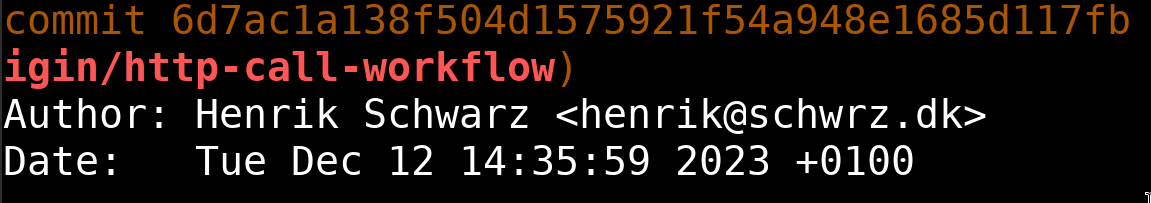
\includegraphics[width=0.5\textwidth]{img/git-commit.png}
    \caption{Commit from developer pushing new code to the project.}
    \label{fig:git-commit}
\end{figure}

Step three in the pipeline is skipped since the project does not have tests. Step four and five are run at 13:36:15 and finish at 13:36:49. Step six of the pipeline is run at 13:36:57 and finishes at 13:37:03. The server is notified when step finishes and then checks if there are any new images which can be seen in figure \ref{fig:server-combined}. Line 1-3 in the figure \ref{fig:server-combined} shows the HTTP request being received and authenticated at 13:36:59 and line 5-8 shows Watchtower stopping, updating, and stating the image for the changed service at 13:37:03. Line 9 shows the status of Watchtower completing the update, stating that there was one service updated and no failures.
\begin{figure}[h]
    \centering
    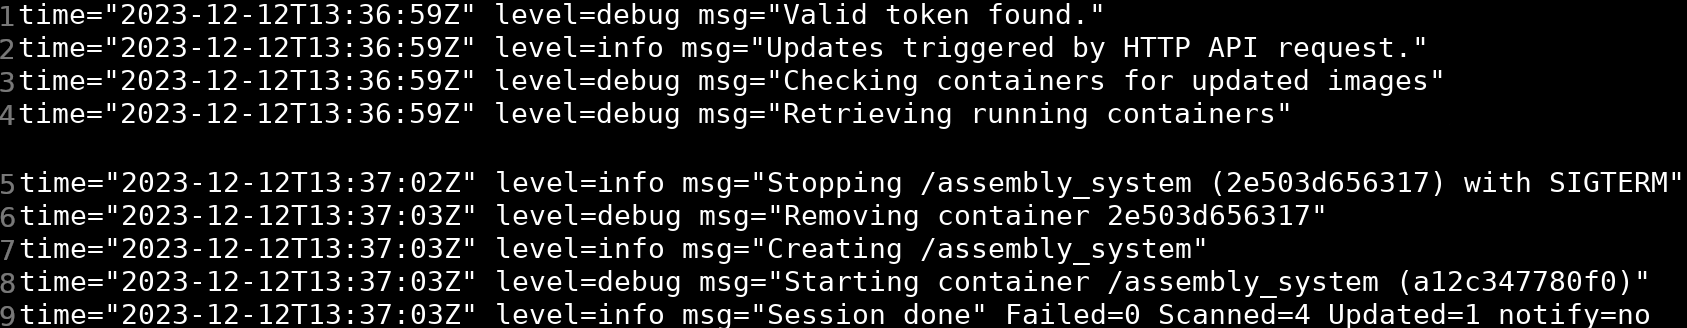
\includegraphics[width=0.5\textwidth]{img/server-combined.png}
    \caption{Combined screenshot of the logs from the server performing the update of the Assembly service.}
    \label{fig:server-combined}
\end{figure}

\subsubsection{Analysis}
To make the analysis easier the timestamps from the measurements from the measurement section have been compiled in table \ref{tab:deployment-measurements}. 'Started' is the started timestamp, 'Completed' is the timestamp for when a step completes, and 'Step time' is the time spent on a step. Step three is omitted since there are no tests. Setup time has been included in the steps.
\begin{table}[h]
\centering
\caption{Table of timestamps from the deployment}
\label{tab:deployment-measurements}
\begin{tabular}{|l|l|l|l|}
\hline
\textbf{Step id} & \textbf{Started} & \textbf{Completed} & \textbf{Step time} \\ \hline
1    & 13:45:39 & 13:45:39 & 0 \\ \hline
2    & 13:36:15 & 13:36:16 & 1 \\ \hline
4    & 13:36:16 & 13:36:43 & 27 \\ \hline
5    & 13:36:43 & 13:36:48 & 5 \\ \hline
6    & 13:36:48 & 13:36:59 & 11 \\ \hline
7    & 13:36:59 & 13:37:03 & 4 \\ \hline
\textbf{Total} & \multicolumn{3}{r|}{48} \\ \hline
\end{tabular}
\end{table}
The deployment process for a small change in a service is adequate being at 48 seconds from commit to live on the server. The time could be more accurate if the project had tests and integration tests since these could increase the time for the pipeline due to having to set up services. Still, the test is an acceptable way to verify the deployability of the system but could have been improved by using more sophisticated orchestration tooling. That would have allowed for testing other interesting deployability tactics such as rollouts and scaling rollouts of the software.
\section{Future work}

Using the QAS for measuring the qualities of an architecture can help to overcome several architectural challenges that will likely drive future work in this field. Such as scalability and performance, interoperability and standardization, deployability, and maintainability.

\subsection{Scalability and Performance}
There are several potential areas for future work related to scalability and performance in Industry 4.0 systems. These include the development of new approaches to leverage brokers between services to facilitate scalable communication. This ensures that all of the communicating services can run with multiple instances simultaneously, leading to the possibility of horizontal scaling. More evaluation is needed of the proposed middleware software architecture design in realistic equipment in the I4.0 lab. This evaluation aims to analyze its scalability and performance against the stated QA requirement.

Moreover, the exploration of new approaches to load balancing is needed to improve scalability and performance in Industry 4.0 systems. This could involve investigating new load-balancing algorithms or developing new load-balancing strategies that are better suited to the unique requirements of Industry 4.0 systems. Additionally, there is a need for investigation into the use of new technologies, such as edge computing \cite{edge-and-fog}, to improve scalability and performance in Industry 4.0 systems. Edge computing involves processing data closer to the source of the data, which can reduce latency and improve performance 

\subsection{Interoperability and Standardization}
Interoperability and standardization in Industry 4.0 systems require, for instance, the development of new approaches to handle the vast amount of data produced by sensors and other IoT devices in Industry 4.0. This could involve exploring new data processing methods, developing standards for data exchange, and evaluating the proposed quality model based on the \textbf{ISO/IEC 25010} standard to identify quality attributes \cite{ANTONINO2022101801} in I4.0 software architectures.

Furthermore, investigation into the use of new technologies such as blockchain to improve interoperability and standardization in Industry 4.0 systems. Blockchain technology \cite{9069885} is a decentralized and secure system that enables transparent data exchange and communication which could be used to create a decentralized, secure, and transparent system for data exchange and communication.

\subsection{Deployability}
In future work, there is an opportunity to explore enhanced deployability through automated deployment techniques, utilizing tools like cloud computing to streamline the deployment process. This could involve investigating new automation strategies and tools to improve the deployability of Industry 4.0 systems and investigation into the use of \textbf{infrastructure as code (IaC)} and configuration management tools \cite{8919181} to improve deployability in Industry 4.0 systems. IaC allows for the automation of infrastructure provisioning and configuration, which can enhance the deployability of software systems.

Moreover, the exploration of new technologies and methodologies for continuous integration and continuous deployment (CI/CD) is essential to improve deployability in Industry 4.0 systems. This could involve investigating new CI/CD tools \cite{7884954}, best practices, and strategies for streamlining the deployment process. Further evaluation of the proposed \textbf{Scripted Deployment Command} tactic and its effectiveness in achieving deployability in Industry 4.0 systems. This could involve testing the strategy in real-world production environments and analyzing its impact on deployment efficiency and system reliability.

\subsection{Maintainability}
 Potential future work related to the quality attribute of maintainability in Industry 4.0 systems may include further investigation into the use of modular and encapsulated software components to improve maintainability in Industry 4.0 systems. This could involve exploring new ways to design and structure software components to facilitate easier maintenance and updates Also investigation of the use of automated testing and continuous monitoring techniques \cite{LEE2006476} to improve maintainability in Industry 4.0 systems, could be beneficial. This could involve exploring new testing methodologies, automated monitoring tools, and strategies for detecting and addressing maintenance issues proactively.

 Furthermore, the exploration of new technologies and methodologies for automated error detection and recovery \cite{s20010109} is essential to improve maintainability in Industry 4.0 systems. This could involve investigating new approaches to detecting and handling errors in real-time, as well as developing automated recovery mechanisms to minimize system downtime and further evaluation of the proposed architectural prototypes and their effectiveness in achieving maintainability in Industry 4.0 systems. This could involve testing the prototypes in real-world scenarios and analyzing their impact on the ease of maintenance, system reliability, and overall system performance.

\section{Conclusion}
Industry 4.0 still has aspects that need to be explored further. This paper looked at the case of an automated fictional bike factory that uses Industry 4.0 and identified four interesting quality attributes: scalability, maintainability, interoperability and deployability. The quality attributes and their meaning for Industry 4.0 was investigated using architectural prototypes and tested via experiments for scalability and deployability which both provided insight into the efficacy of the architecture. The scalability experiment raised interesting insights that would need further experimentation on bottlenecks between the supervisor system and InfluxDB and the deployability experiment verified the deployment solution for the architecture using the cycle time for a deployment. 
Further work could be done on the scalability of the architecture by also including the scaling of the broker and databases and the deployability of the system could be investigated further by looking at the other deployability tactics mentioned in the analysis section of experiment B. In the future, further work should investigate how architectural prototypes can contribute to verifying Industry 4.0 architectures and also answer if the technology choices and their limitations should be considered earlier in the process or together with the quality attributes and QAS.

\bibliographystyle{IEEEtran}
\bibliography{references}
\vspace{12pt}
\end{document}
